% ===== 原文 pp.1–17（PDF pp.8–24） =====
% [原文 p.1]
\chapter{背景与概观}

本章叙述本书所讨论的导出范畴、三角范畴、$A_\infty$ 范畴以及它们之间关系之数学的与物理的背景。将出现大量专门术语，读者即使不知道也无妨；必要的内容将在第 2 章以后定义。

\section{引言}

所谓范畴（圏），指的是由称为对象（対象）的数学对象构成的族，与它们之间的态射（射，即映射）构成的族，且满足适当条件者。例如，集合所构成的范畴 $\Set$，是以每个集合为对象，对两个对象即集合 $A,B$，以映射 $f\colon A\to B$ 为从 $A$ 到 $B$ 的态射而得到的范畴。与映射的合成相对应的态射的合成在范畴中被定义，关于合成的结合律等也包含在范畴定义中的「适当条件」之内。此外，范畴的例子还有拓扑空间（topological space）的范畴 $\Top$、加法群（Abelian group）的范畴 $\Ab$ 等。

% [Tutor Note: 原文 p.1「圏とは，対象と呼ばれる数学的対象の集まりと，それらの間の射（写像）達であって，適切な条件を満たすもの」为范畴的直观描述，正式定义见第 4 章 定義 4.1；此处「集まり」不宜译「集合」（避免与 ZFC 意义下的集合混淆），故译「族」。]

另一方面，对于几何对象，例如拓扑空间、流形以及带各种结构的流形等，存在使其对应于范畴的标准方法；只要在范畴之间定义了适当的等价关系，就可以期待把范畴作为（带结构的）拓扑空间的某种不变量来应用。例如，通过拓扑空间 $X$ 上的向量丛所构成的范畴而确定的 $K_0$ 群便是其例。现在，关于复流形或代数簇 $X$ 上的相干层（coherent sheaf）所构成的范畴 $\mathit{coh}(X)$ 的研究也很兴盛。在这个例子中，依 $X$ 的不同，已处于可以了解范畴 $\mathit{coh}(X)$ 所具有的结构之细节的水平，并在 $\mathit{coh}(X)$ 上展开某种同调代数。特别地，通过对 $\mathit{coh}(X)$ 施加某种同调代数操作而得到的导出范畴，是主要研究对象之一。同样地，作为可以定义导出范畴并处于能够研究其结构的水平者，还有有限维代数 $A$ 上的模所构成的范畴 $\mathrm{mod}\text{-}A$ 等。

% [Tutor Note: 原文 p.1「圏の射」译「态射」而不译「映射」，是因为范畴中的射一般不必是映射（例如偏序集视为范畴时，射是序关系；关系范畴 $\mathbf{Rel}$ 的射是关系）。$\Set$ 的射恰为映射、$\Top$ 的射为连续映射、$\Ab$ 的射为群同态，这只是特例。]

% [Tutor Note: 原文 p.1「ベクトル束らの成す圏を通して定まる $K_0$ 群」补出作者省略的构造（可验证锚点）：对紧拓扑空间 $X$，$K_0(X)$ 由 $X$ 上复向量丛的同构类 $[E]$ 生成，并对每个短正合列 $0\to E'\to E\to E''\to 0$ 施加关系 $[E]=[E']+[E'']$（即 Grothendieck 群构造）。取 $X$ 为一点时 $K_0(\mathrm{pt})=\mathbb{Z}$（由秩给出），这是核对此构造的最简单例子。]

% [原文 p.2]
Kontsevich 的同调镜像对称（homological
mirror symmetry）猜想 [37] 进一步激活了此类同调代数的范畴论研究。镜像对称性一般是指复流形与辛流形之间成立的（各种层面的）对偶性 [20]，而同调镜像对称则是它们之间的范畴论对偶性，被表述为称为 Fukaya 范畴的、由辛流形中的拉格朗日子流形等所构成的范畴，与复流形上的相干层所构成的范畴 $\mathit{coh}(X)$ 之间的某种范畴等价（[20]）。在这些范畴中，对象一般有无限多个（即使模去同构），并且依所讨论的范畴等价处于哪个层面而定，实际已被证明同调对称性的例子（辛流形与复流形的配对）还不多。但是，当范畴的性质在一定程度上足够好、例如能取到由有限个对象构成的某种生成系时，只需在该生成系之间进行比较即可。也就是说，若两个范畴具有等价的生成系，则范畴等价随之成立。在这种情形下，该生成系附带自然的环（代数）结构，于是第三个范畴——该代数上的模的范畴——便出现了。也就是说，在讨论同调镜像对称时，作为其中间步骤，也会出现某个环（或其扩张）$A$ 上的模的范畴 $\mathrm{mod}\text{-}A$。

% [Tutor Note: 原文 p.2「2 つの圏が同値な生成系を持てば，圏同値が従う」补出省略论证：设 $\cC,\cD$ 分别由生成系 $\{E_i\}$、$\{F_i\}$ 生成，且存在同一指标集上的对象对应 $E_i\mapsto F_i$ 及相容的态射对应；则全子范畴 $\langle E_i\rangle$、$\langle F_i\rangle$ 之间的函子在生成系上给出全忠实且本质满（本质满由生成系张成整个范畴保证），从而为范畴等价。最简可验证的例子即本书 p.5 提到的 $\Db(\mathit{coh}(\C P^1))$：其例外生成系 $\{\cO,\cO(1)\}$ 满足 $\End(\cO\oplus\cO(1))$ 为 Kronecker 箭图的路代数（例 6.24）。]

% [Tutor Note: 原文 p.2 末「環（やその拡張）$A$ 上の加群の圏 $\mathrm{mod}\text{-}A$」中 $\mathrm{mod}\text{-}A$ 指「有限生成右 $A$ 模」的范畴（第 2 章定义，第 6 章 p.145 起系统使用）；此处译「模的范畴」并保留记号，preamble 已定义 \verb|\modA|，本块按原书排印写作 $\mathrm{mod}\text{-}A$ 以与样板一致。]

本书就这种范畴论的同调代数侧面，仅假定线性代数的知识而展开讨论。对于导出范畴、以导出范畴为典型例的三角范畴，以及定义 Fukaya 范畴时也需要的 $A_\infty$ 范畴，本书力求尽可能直截了当地使读者习得。导出范畴与三角范畴是只知其定义并不能真正理解的抽象对象，因此，为了理解导出范畴的定义之意义与其在应用上的重要性，本书把性质良好的有限维代数 $A$ 上的模的范畴 $\mathrm{mod}\text{-}A$ 的导出范畴置于例子的中心。

另一方面，关于这些范畴论的同调代数在上述意义上的几何背景，正文（第 2 章以后）不予讨论。例如，作为导出范畴最基本的例子之一的、复流形或代数簇上的相干层所构成的导出范畴，本书不予讨论。这是因为，从线性代数开始一直定义到相干层，还需要更多篇幅。然而，导出范畴是从阿贝尔范畴出发施加本书所说明的那种操作而得到的，所以只要知道相干层构成阿贝尔范畴 $\mathit{coh}(X)$，便可得到 $\Db(\mathit{coh}(X))$。对相干层所构成的阿贝尔范畴 $\mathit{coh}(X)$ 作出说明的书籍，日语教科书中也有若干（例如，小林 [36]，Iversen（前田译）[23]）。反之，对于以这些几何为背景讨论同调镜像对称时近年来发展起来的纯同调代数方法，本书作了相当详细的讨论。大体上说，作为三角范畴，由某个 DG 范畴、或更一般地由 $A_\infty$ 范畴得到的居多。例如导出范畴即是其例。另一方面，已知也有并非如此的例子（Muro et al. [45]）。把这样的例子看作例外而有趣的东西，还是看作性质恶劣的三角范畴，或许因人而异。

% [原文 p.3]
但本书对由 DG 范畴与 $A_\infty$ 范畴得到的三角范畴所具有的性质作了相当详细的讨论，这也是本书的特色之一。

% [Tutor Note: 术语首现对照（p.2–p.3）：導来圏 = 导出范畴 derived category；三角圏 = 三角范畴 triangulated category；連接層 = 相干层 coherent sheaf；生成系 = 生成系 generating set；ミラー対称性 = 镜像对称 mirror symmetry；深谷圏 = Fukaya 范畴 Fukaya category。]

\section{本书的构成}

第 2 章总结了本书所讨论题材相关的基本语言与工具。加法群（＝模＝阿贝尔群）几乎是所有章节都需要的。此外，固定环 $R$ 时的 $R$ 模，及其特别情形即 $R$ 为域 $K$ 时的 $K$ 向量空间等，作为日后讨论导出范畴、三角范畴、$A_\infty$ 范畴等时的具体例子也很重要。其他方面，第 2 章还讨论了定义导出范畴时所需的、作为范畴论中局部化之基础概念的环的局部化；不过这一部分可以一开始跳过，等到范畴的局部化（4.7 节）中在意时再回来读。加法群或 $R$ 模的直和本身是基本的东西，但最好也从「它是范畴论中直和的例子」这一意义上去理解。关于张量积，直到讨论 $A_\infty$ 范畴或 $A_\infty$ 代数为止都不会用到。代数除了 $A_\infty$ 代数之外，还在第 6 章讨论有限维代数时需要。

% [Tutor Note: 原文 p.3「加法群（＝加群＝アーベル群）」给出术语锚点：本书把 $\Z$ 模、加法群、阿贝尔群视为同一对象（第 2 章统一处理）。核对方法：任一阿贝尔群 $M$ 上 $n\cdot m$（$n\in\Z$）由群运算唯一确定，故 $M$ 恰为 $\Z$ 模；故此三词在本书可互换。]

第 3 章讨论加法群与 $R$ 模（含向量空间）的同调代数，特别是复形、正合列、复形的同伦等。这些是导出范畴、三角范畴这两个概念的基础背景，所以最好熟悉之；它们也成为导出范畴、三角范畴中所出现的结构的例子。

第 4 章定义导出范畴。导出范畴是从范畴中在如第 3 章所讨论的同调代数操作下封闭这一意义上性质良好的阿贝尔范畴 $\cC$ 出发，按以下步骤定义的。

\begin{itemize}
\item 构成以 $\cC$ 中各个复形为对象的范畴 $\Comp(\cC)$。
\item 用复形的同伦去除 $\Comp(\cC)$ 的态射，得到同伦范畴 $\mathrm{K}(\cC)$。
\item 用 $\mathrm{K}(\cC)$ 的拟同构映射对 $\mathrm{K}(\cC)$ 作（范畴论意义下的）局部化。
\end{itemize}

这样得到的范畴称为阿贝尔范畴 $\cC$ 的导出范畴 $\mathrm{D}(\cC)$。也就是说，只要有阿贝尔范畴，导出范畴就总能定义。然而，关于「可以用拟同构映射进行局部化」这一事实的证明，由于着眼于下一章所讨论的同伦范畴 $\mathrm{K}(\cC)$ 所具有的三角结构最为明快，故放到那里处理。

% [Tutor Note: 原文 p.3 的三步骤把导出范畴刻画为 $\mathrm{D}(\cC)=\mathrm{K}(\cC)[\Sigma^{-1}]$（$\Sigma$ 为拟同构的类）。可验证的锚点：$\mathrm{D}(\cC)$ 与 $\mathrm{K}(\cC)$ 有相同的对象（都是 $\cC$ 的复形），差别只在态射——$\mathrm{D}(\cC)$ 的态射由「屋顶」$X\xleftarrow{\ \sim\ } Z\to Y$（左端为拟同构）表示，见 4.7 节与定理 4.58。注意 $X,Y$ 在 $\mathrm{K}(\cC)$ 中不同构而在 $\mathrm{D}(\cC)$ 中同构，正是局部化「扩大态射空间」的效果。]

第 5 章说明三角范畴这一概念。对阿贝尔范畴 $\cC$ 所构成的同伦范畴 $\mathrm{K}(\cC)$ 与导出范畴 $\mathrm{D}(\cC)$ 是三角范畴的典型例。反过来说，三角范畴可以说是把导出范畴 $\mathrm{D}(\cC)$ 及其基础同伦范畴 $\mathrm{K}(\cC)$ 所具有的基本性质作为公理系抽取出来的东西（Verdier）。例如导出范畴的等价性，就被表述为作为三角范畴的等价性。

另一方面，三角范畴的定义（公理）是那种只记住它并不能说就理解了三角范畴的东西。也就是说，公理越简单越美。正因如此，三角范畴也（虽说很难说非常单纯）由最小限度的公理系定义，而从该公理可推出各种可称为更基本的性质。

% [原文 p.4]
5.1 节首先在 5.1.1 节直截了当地叙述三角范畴的公理，然后在 5.1.2 节讨论由该公理推出的各种性质，并思考三角范畴公理的意义。5.2 节确认阿贝尔范畴（或加法范畴）$\cC$ 的同伦范畴 $\mathrm{K}(\cC)$ 构成三角范畴。接着在 5.3 节讨论 $\mathrm{K}(\cC)$ 关于拟同构映射的局部化，并看到 $\mathrm{D}(\cC)$ 构成三角范畴。5.4 节在适当的假设下证明导出范畴与某个加法范畴的同伦范畴等价。为此本书经由定理 5.36、5.42。由于觉得这个过程本身也有几分价值，故也写入了它们证明的细节，不过读者不妨先跳过、只追主张即可。5.5 节叙述由 DG 范畴构造三角范畴。这样得到的三角范畴不仅满足三角范畴的公理，还具有更牢固的结构。也就是说，三角范畴的结构被增广了。特别地，同伦范畴具有 DG 增广。

% [Tutor Note: 原文 p.4「このために本書では定理 5.36, 5.42 を経由する」为编号核对锚点：这两条定理属于第 5 章 5.4 节（原书 pp.106–124，由负责该块的译者处理）；本块只照录编号，不展开内容。]

5.6 节、5.7 节讨论关于不假定 DG 增广存在的一般三角范畴中的附加结构、由 Bondal 等人发展起来的理论。

% [Tutor Note: 术语「DG 増強」译「DG 增广」（DG enhancement）。可验证锚点：对加法范畴 $\cC$，其同伦范畴 $\mathrm{K}(\cC)$ 的 Hom 集可升级为 Hom 复形 $\Hom^\bullet(X,Y)$（上链复形），复合满足 Leibniz 规则，于是 $\mathrm{K}(\cC)$ 成为三角 DG 范畴；若把 $\mathrm{K}(\cC)$ 换成只含某类对象的全子范畴（如投射对象的同伦范畴），DG 结构限制过去即得 DG 增广。]

第 6 章作为导出范畴（也就是三角范畴）的例子，讨论有限维代数（也就是环）$A$ 上的模所构成的阿贝尔范畴 $\mathrm{mod}\text{-}A$ 的导出范畴 $\Db(\mathrm{mod}\text{-}A)$。应用 5.5 节的 DG 增广理论、5.6 节与 5.7 节讨论的理论，讨论在性质良好的有限维代数 $A$ 情形下导出范畴 $\Db(\mathrm{mod}\text{-}A)$ 所具有结构的一般理论，同时在若干例子中具体求出阿贝尔范畴 $\mathrm{mod}\text{-}A$ 与导出范畴 $\Db(\mathrm{mod}\text{-}A)$ 的对象与态射。

第 7 章讨论 $A_\infty$ 范畴，以及由 $A_\infty$ 范畴构造三角范畴的方法。7.1 节说明 $A_\infty$ 代数的定义与性质。$A_\infty$ 范畴是作为 $A_\infty$ 代数的自然扩张而定义的，其性质也作为 $A_\infty$ 代数所具有的各种性质来理解。关于由 $A_\infty$ 范畴得到的三角范畴，讨论从 $A_\infty$ 代数所具有的同伦结构导出的各种性质。7.4 节讨论 $A_\infty$ 结构的米田嵌入，它使得可以对 $A_\infty$ 结构定义与之 $A_\infty$ 同伦等价的 DG 结构。由此便可以在 DG 范畴与 $A_\infty$ 范畴之间自由往返，可知在一侧成立的事情在另一侧也成立。最后在 7.5 节举出几个 $A_\infty$ 代数、$A_\infty$ 范畴的例子。

以下，1.3 节概述第 2 章以后所讨论内容的背景，1.4 节概述它们与弦理论的关联，1.5 节概述第 2 章以后所展开讨论的技术性侧面。

% [Tutor Note: 原文 p.4「米田埋め込み」= 米田嵌入 Yoneda embedding（正文作「米田埋め込み」，见 7.4 节）。可验证锚点：嵌入 $A\mapsto \Hom_{A_\infty}(-,A)$ 把 $A_\infty$ 代数/范畴送入 $A_\infty$ 函子范畴，其像上的 Hom 复形给出 DG 结构；这是 7.4 节把 $A_\infty$ 结构「DG 化」的机制。]

% [原文 p.5]
\section{理论的数学背景}

\subsection{导出范畴与三角范畴}

如前所述，对于在同调代数操作下封闭这一意义上性质良好的阿贝尔范畴 $\cC$，作为其复形范畴 $\Comp(\cC)$ 的同伦范畴 $\mathrm{K}(\cC)$ 的局部化，定义导出范畴 $\mathrm{D}(\cC)$；而把同伦范畴 $\mathrm{K}(\cC)$ 与导出范畴 $\mathrm{D}(\cC)$ 所具有的基本性质公理化得到的概念，就是三角范畴。更具体地说，三角范畴 $\cT$ 是指某个加法范畴，它带有自同构 $\T\colon \cT\to\cT$，并带有由某个公理系所定义的正合三角序列（exact triangle）。这里，正合三角序列是指 $\cT$ 中的某个序列

\[\cdots \T^{-1}(Z)\xrightarrow{\T^{-1}(w)} X\xrightarrow{u} Y\xrightarrow{v} Z\xrightarrow{w} \T(X)\xrightarrow{\T(u)} \T(Y)\xrightarrow{\T(v)} \T(Z)\xrightarrow{\T(w)} \cdots\]

由该式可以明白，$(X,Y,Z;u,v,w)$ 构成上述正合三角序列时，$(Y,Z,\T(X);v,w,\T(u))$ 也构成正合三角序列，这一点包含在该公理之中。特别地，对 $\cT$ 中任意态射 $u\colon X\to Y$，如上那样的正合三角序列必定存在，且其对象 $Z\in\cT$ 在模同构的意义下被唯一确定。在三角范畴中，由这样的正合三角序列可得长正合列，它例如给出计算态射空间维数等的同调代数手段。在本书中，5.6.1 节等处可以看到其应用例。

% [Tutor Note: 原文 p.5 的「旋转」性质即公理 (Tr2)：$(X,Y,Z;u,v,w)$ 为正合三角序列时 $(Y,Z,\T(X);v,w,\T(u))$ 亦然。可验证锚点：书中的 $\T$ 与记号 $[1]$ 是同一个平移函子，反复旋转三次回到原序列（同构意义下）。]

导出范畴最重要的例子之一，是代数簇或复流形 $M$ 上的相干层所构成的阿贝尔范畴 $\mathit{coh}(M)$ 的导出范畴 $\Db(\mathit{coh}(M))=:\Db(M)$。例如复射影空间 $\C\mathrm{P}^n$ 上的相干层的导出范畴 $\Db(\C\mathrm{P}^n)$ 所具有的结构可由某个箭图来描述（Beilinson [6]）。特别地，$\Db(\mathit{coh}(\C\mathrm{P}^1))$ 与由 Kronecker 箭图（例 6.24）所描述的代数（环）上的模的范畴的导出范畴作为三角范畴等价。

% [Tutor Note: 可验证锚点（Beilinson）：$\Db(\mathit{coh}(\C\mathrm{P}^n))$ 由线丛 $\{\cO,\cO(1),\dots,\cO(n)\}$ 生成（例外对象系），且 $\Hom(\cO(i),\cO(j))=\mathrm{Sym}^{j-i}(\C^{n+1})$；由此 $\End(\bigoplus_{i=0}^{n}\cO(i))$ 为 $(n+1)$ 个顶点、相邻顶点间有 $n+1$ 重箭头的箭图的路代数（$n=1$ 时即 Kronecker 箭图，两个顶点、两重箭头），本书 p.5 所谓「由 Kronecker 箭图描述的代数」即此。]

在这样的讨论中，关键在于找到可视为三角范畴生成系的对象。在这样的生成系之中，有作为 $\Db(\mathit{coh}(\C\mathrm{P}^1))$ 的生成系所具有性质的推广的（强）例外生成系（(strongly) exceptional collection），关于它的一般理论已由 Bondal 等人展开 [7]。

另一方面，作为可称为紧流形的 Poincaré 对偶性的复流形版、范畴版的东西，对于光滑紧射影代数簇 $M$，导出范畴 $\Db(M)$ 具有称为 Serre 对偶性的对偶性。这样的对偶性对于理解导出范畴的结构之强有力，是不言而喻的。这种 Serre 对偶性被重新表述到一般三角范畴的情形 [9]。特别地，三角范畴若具有例外生成系，则具有 Serre 对偶性（定理 5.74）。本书在 5.6 节讨论关于例外生成系的一般理论，在 5.7 节讨论 Serre 对偶性。这些内容在第 6 章被应用于关于性质良好的有限维代数 $A$ 上的模的导出范畴 $\Db(\mathrm{mod}\text{-}A)$ 的结构的讨论。

% [Tutor Note: 术语与定义锚点：Serre 对偶由 Serre 函子 $\nu\colon \Db(M)\to\Db(M)$ 与自然同构 $\Hom(X,Y)\cong\Hom(Y,\nu X)^{*}$ 给出（$\nu=\omega_M\otimes -$ 的导出函子，移位 $\dim M$）。定理 5.74 的编号属第 5 章 5.7 节（原书 pp.125–144），本块仅照录编号；此处「例外生成系 $\Rightarrow$ Serre 对偶」是 5.7 节的主结论。]

话虽如此，只要有阿贝尔范畴，其导出范畴就能定义，因此可以构成各种各样的导出范畴；本书所讨论的不过是其中的一例。

% [原文 p.6]
其他例如，对于 D 模（由线性微分算子所构成的模）的阿贝尔范畴，可以考察其导出范畴 [34]。作为有限群论中的应用，关于有限群的群环的模的阿贝尔范畴的导出范畴的结构研究也在进行。

\subsection{什么是 $A_\infty$ 代数结构？}

固定域 $K$ 时，$K$ 上的代数 $A$ 是指 $K$ 上向量空间带有乘法结构而构成环者（定义 2.71）。乘法是指从 $A$ 的两个元素给出一个 $A$ 的元素的对应。$A_\infty$ 代数是代数的推广。$A$ 上的 $A_\infty$ 结构，是指从 $A$ 的 $k$ 个元素给出一个 $A$ 的元素的对应所构成的族

\[\{m_k : A\times\cdots\times A\to A\}_{k=1,2,\ldots}\]

且对每个 $n=1,2,\ldots$ 满足关系式

\begin{equation}
\sum_{k+l=n+1}\sum_i \pm m_k(a_1,\ldots,a_i,m_l(a_{i+1},\ldots,a_{i+l}),\ldots,a_n)=0 \tag{1.1}
\end{equation}

者。更准确地说，此时若 $A$ 是分次向量空间、且各 $m_k$ 是次数 $(2-k)$ 的多重线性映射，则称 $(A,\{m_k\}_{k\ge1})$ 为 $A_\infty$ 代数（$A_\infty$-algebra）。这样的 $A_\infty$ 结构，最初是在同伦论中作为加于拓扑空间之上的结构而由 Stasheff 引入的 [50]。作为典型例子，带基点圈空间上 $A_\infty$ 结构如下自然地确定。对拓扑空间 $X$ 与基点 $x_0\in X$，带基点圈 $x$ 是指满足 $x(0)=x(1)=x_0$ 的连续映射 $x\colon[0,1]\to X$。由带基点圈所构成的空间称为带基点圈空间，记作 $Y=\Omega X$。给定两个带基点圈时，把它们接合并将长度减半，便再次得到带基点圈（图 1.1(a)）。由此，积

\[M_2 : Y\times Y\to Y\]

被定义。

% [Tutor Note: 原文 p.6 式 (1.1) 中的 $\pm$ 由 Koszul 符号规则决定（对次数为 $|a|$ 的元素，交换时产生 $(-1)^{|a||b|}$）。可验证的锚点（正文 p.9 明言）：$n=1$ 时求和只剩 $k=l=1$、$i=1$ 一项，得 $m_1(m_1(a_1))=0$，即 $(m_1)^2=0$；$n=2$ 给出 $m_1$ 关于 $m_2$ 的 Leibniz 法则；$n=3$ 给出 $m_2$ 的同伦结合性。]

% [Tutor Note: 原文 p.6「各 $m_k$ が次数 $(2-k)$ の多重線形写像」给出次数约定的锚点：$k=1$ 时次数为 $1$（微分），$k=2$ 时次数为 $0$（乘法），与 p.9 所说「次数 $(2-n)$ 的 $A_\infty$ 構造 $m_n$」一致；这也解释了为什么 $m_1$ 是微分而 $m_2$ 是通常的乘法。]

\begin{center}
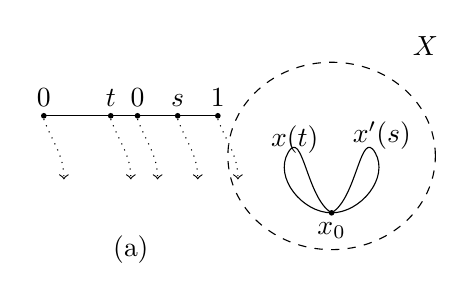
\begin{tikzpicture}[scale=0.85]
  % (a) 两个参数区间
  \draw (0,0)--(2.6,0);
  \foreach \x/\lab in {0/0, 1.0/t, 1.4/0, 2.0/s, 2.6/1} { \fill (\x,0) circle (1.2pt); \node[above] at (\x,0) {$\lab$}; }
  \foreach \x in {0,1.0,1.4,2.0,2.6} { \draw[->,dotted] (\x,-0.05) to[out=-70,in=90] (\x+0.3,-0.95); }
  % 带基点圈空间 X
  \draw[dashed] (4.3,-0.6) ellipse (1.55 and 1.4);
  \node[above] at (5.7,0.75) {$X$};
  \fill (4.3,-1.45) circle (1.2pt) node[below] {$x_0$};
  \draw (4.3,-1.45) to[out=150,in=60] (3.65,-0.55) to[out=-120,in=180] (4.3,-1.45);
  \draw (4.3,-1.45) to[out=30,in=120] (4.95,-0.55) to[out=-60,in=0] (4.3,-1.45);
  \node at (3.75,-0.35) {$x(t)$};
  \node at (5.05,-0.3) {$x'(s)$};
  \node at (1.3,-2.0) {(a)};
\end{tikzpicture}\qquad
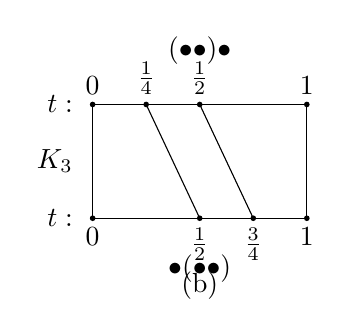
\begin{tikzpicture}[scale=0.85]
  \draw (0,0) rectangle (3.2,1.7);
  \foreach \x/\lab in {0/0, 0.8/\frac14, 1.6/\frac12, 3.2/1} { \fill (\x,1.7) circle (1.2pt); \node[above] at (\x,1.7) {$\lab$}; }
  \foreach \x/\lab in {0/0, 1.6/\frac12, 2.4/\frac34, 3.2/1} { \fill (\x,0) circle (1.2pt); \node[below] at (\x,0) {$\lab$}; }
  \draw (0.8,1.7)--(1.6,0);
  \draw (1.6,1.7)--(2.4,0);
  \node[left] at (-0.15,0.85) {$K_3$};
  \node[left] at (-0.15,1.7) {$t:$};
  \node[left] at (-0.15,0) {$t:$};
  \node[above] at (1.6,2.15) {$(\bullet\bullet)\bullet$};
  \node[below] at (1.6,-0.4) {$\bullet(\bullet\bullet)$};
  \node at (1.6,-1.0) {(b)};
\end{tikzpicture}

{\small \textbf{图 1.1}\quad (a) 带基点的圈的积。(b) $(\bullet\bullet)\bullet := M_2(M_2(\bullet,\bullet),\bullet)$ 与 $\bullet(\bullet\bullet) := M_2(\bullet,M_2(\bullet,\bullet))$ 之间的同伦。这里 $\bullet$ 分别表示 $Y$ 的元。\par}
\end{center}

% [原文 p.7]
该积并不结合，但 $M_2(M_2\times1), M_2(1\times M_2)\colon Y\times Y\times Y\to Y$ 中带基点圈的参数化可以通过线段 $K_3$ 连接起来（图 1.1(b)）。由此，映射

\[M_3 : K_3\times Y\times Y\times Y\to Y\]

被定义。如图 1.2(a) 所示，把 $M_2,M_3$ 等结构用树图表示便容易理解。类似地，考虑由 $M_2$ 与 $M_3$ 构成的映射 $(Y)^{\times4}\to Y$。它们构成五边形的边界，而由带基点圈的性质，该映射可以延拓到五边形内部（图 1.2(b)）。如此得到 $M_4 : K_4\times Y^{\times4}\to Y$，再重复此操作，便得到 $(n-2)$ 维多面体 $K_n$ 与映射

\[M_n : K_n\times (Y)^{\times n}\longrightarrow Y\]

关于 $n=2$，规定 $K_2=\{\text{一点}\}$。

把具有这种性质的映射之族 $\{M_n : K_n\times Y^{\times n}\to Y\}$ 作为附加结构的拓扑空间 $Y$，称为 $A_\infty$ 空间（$A_\infty$-space）[50]。多面体 $K_n$ 称为 Stasheff associahedron，或简称为 Stasheff 多面体（Stasheff polyhedron）。前一个名字意味着，对 $K_n$ 的每个胞腔都附随了与结合律（associativity）相关的树图（associated）。例如，$K_4$ 的 2 维胞腔对应叶为 4 片、顶点为 1 个的树；5 个 1 维胞腔（五边形的周边）分别对应叶为 4 片、顶点为 2 个的树；5 个 0 维胞腔（五边形的顶点）分别对应叶为 4 片、顶点为 3 个的树。一般地，$K_n$ 的 $i$ 维胞腔附随叶为 $n$ 片、顶点为 $(n-i+1)$ 个的树。

% [Tutor Note: 原文可疑处（p.7，正誤表未收）：紧接上文的例子对 $n=4$ 给出 $i=2,1,0$ 时顶点数分别为 $1,2,3$，这与通式 $(n-i+1)$ 不符（$i=2$ 时通式给 $3$，$i=0$ 时给 $5$）。按例子反推，通式应为 $(n-i-1)$；本译本照印文译出，未擅改。可验证：$K_3$ 是线段（1 维），对应 $n=3,i=1$，例子体系下的公式给 $3-1-1=1$ 个顶点（即一条边的树），与图 1.2(a) 一致。]

\begin{center}
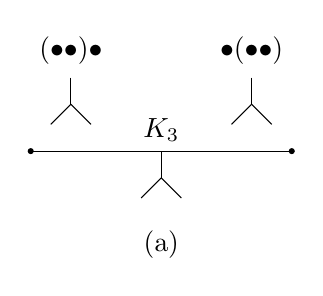
\begin{tikzpicture}[scale=0.85]
  \node at (0.6,2.0) {$(\bullet\bullet)\bullet$};
  \node at (3.3,2.0) {$\bullet(\bullet\bullet)$};
  \draw (0.6,1.6)--(0.6,1.2); \draw (0.6,1.2)--(0.3,0.9); \draw (0.6,1.2)--(0.9,0.9);
  \draw (3.3,1.6)--(3.3,1.2); \draw (3.3,1.2)--(3.0,0.9); \draw (3.3,1.2)--(3.6,0.9);
  \draw (0,0.5)--(3.9,0.5); \fill (0,0.5) circle (1.3pt); \fill (3.9,0.5) circle (1.3pt);
  \node[above] at (1.95,0.5) {$K_3$};
  \draw (1.95,0.5)--(1.95,0.1); \draw (1.95,0.1)--(1.65,-0.2); \draw (1.95,0.1)--(2.25,-0.2);
  \node at (1.95,-0.9) {(a)};
\end{tikzpicture}\qquad
\begin{tikzpicture}[scale=0.85]
  \coordinate (P1) at (0.3,1.1); \coordinate (P2) at (1.3,1.9); \coordinate (P3) at (2.6,1.9);
  \coordinate (P4) at (3.6,1.1); \coordinate (P5) at (2.8,0); \coordinate (P6) at (1.1,0);
  \fill[gray!35] (P1)--(P2)--(P3)--(P4)--(P5)--(P6)--cycle;
  \draw (P1)--(P2)--(P3)--(P4)--(P5)--(P6)--cycle;
  \foreach \p in {P1,P2,P3,P4,P5,P6} { \fill (\p) circle (1.3pt); }
  \node at (2.45,0.6) {$K_4$};
  \foreach \a in {50,70,90,110} { \draw ($(2.0,0.95)+(\a:0.08)$) -- ($(2.0,0.95)+(\a:0.5)$); }
  \foreach \x/\y in {1.3/2.45, 2.6/2.45, 0.25/1.7, 3.65/1.7, 0.45/0.6, 3.45/0.6, 1.1/-0.5, 2.8/-0.5, 1.95/-0.55, -0.2/1.1, 4.05/1.1} {
    \draw (\x,\y)--(\x,\y+0.3); \draw (\x,\y+0.3)--(\x-0.18,\y+0.55); \draw (\x,\y+0.3)--(\x+0.18,\y+0.55);
  }
  \node at (1.95,-1.2) {(b)};
\end{tikzpicture}

{\small \textbf{图 1.2}\quad (a) Stasheff 多面体 $K_3$（线段）。(b) Stasheff 多面体 $K_4$（五边形）。\par}
\end{center}

集合族 $\{K_n\}$ 所具有的结构，由称为 operad 的概念来说明。

% [原文 p.8]
\begin{center}
\begin{tikzpicture}[scale=0.8]
  % 左：O(k) (i) O(l) (j) O(m)
  \node[draw,circle,inner sep=1pt] (K1) at (0,0) {$\mathcal{O}(k)$};
  \node[draw,circle,inner sep=1pt] (L1) at (2.1,0.15) {$\mathcal{O}(l)$};
  \node[draw,circle,inner sep=1pt] (M1) at (4.2,-0.2) {$\mathcal{O}(m)$};
  \draw[->] (-1.25,0)--(K1);
  \draw (K1)--(L1); \node[above] at (1.05,0.4) {$(i)$};
  \draw (L1)--(M1); \node[above] at (3.2,0.25) {$(j)$};
  \foreach \a/\lab in {55/1, 80/2, -55/k-1, -80/k} {
    \draw ($(K1)+(\a:0.28)$)--($(K1)+(\a:0.72)$); \node at ($(K1)+(\a:0.95)$) {$\lab$}; }
  \foreach \a/\lab in {55/1, 80/2, -60/l+m-1} {
    \draw ($(L1)+(\a:0.28)$)--($(L1)+(\a:0.72)$); \node at ($(L1)+(\a:0.95)$) {$\lab$}; }
  \foreach \a/\lab in {45/j, 62/j+1, 79/j+2, -50/j+m-2, -68/j+m-1} {
    \draw ($(M1)+(\a:0.28)$)--($(M1)+(\a:0.72)$); \node at ($(M1)+(\a:0.95)$) {$\lab$}; }
  \draw[dotted,thick] (2.15,0.05) ellipse (1.75 and 1.25);
  \draw[dotted,thick] (3.7,-0.15) ellipse (1.55 and 1.05);
  % 等号
  \node at (6.0,0) {$=$};
  % 右：O(k) (i) O(l) (j') O(m)
  \node[draw,circle,inner sep=1pt] (K2) at (7.6,0) {$\mathcal{O}(k)$};
  \node[draw,circle,inner sep=1pt] (L2) at (9.7,0.15) {$\mathcal{O}(l)$};
  \node[draw,circle,inner sep=1pt] (M2) at (11.9,-0.2) {$\mathcal{O}(m)$};
  \draw[->] (6.35,0)--(K2);
  \draw (K2)--(L2); \node[above] at (8.65,0.4) {$(i)$};
  \draw (L2)--(M2); \node[above] at (10.8,0.3) {$(j')$};
  \foreach \a/\lab in {55/1, 80/2, -55/k-1, -80/k} {
    \draw ($(K2)+(\a:0.28)$)--($(K2)+(\a:0.72)$); \node at ($(K2)+(\a:0.95)$) {$\lab$}; }
  \foreach \a/\lab in {55/1, 80/2, -55/k+l-2, -75/k+l-1} {
    \draw ($(L2)+(\a:0.28)$)--($(L2)+(\a:0.72)$); \node at ($(L2)+(\a:0.95)$) {$\lab$}; }
  \foreach \a/\lab in {55/i, 72/i+1, 30/1, 12/2, -5/3, -55/m-1, -75/m} {
    \draw ($(M2)+(\a:0.28)$)--($(M2)+(\a:0.72)$); \node at ($(M2)+(\a:0.95)$) {$\lab$}; }
  \draw[dotted,thick] (9.75,0.05) ellipse (1.75 and 1.25);
  \draw[dotted,thick] (11.4,-0.15) ellipse (1.55 and 1.05);
\end{tikzpicture}

{\small \textbf{图 1.3}\quad operad $\{\mathcal{O}(n)\}_{n\ge1}$ 及其结合性 $\mathcal{O}(k)\circ_i(\mathcal{O}(l)\circ_j\mathcal{O}(m))=(\mathcal{O}(k)\circ_i\mathcal{O}(l))\circ_{j'}\mathcal{O}(m)$，$j' := (i-1)+j$ 的示意图。\par}
\end{center}

一般地，operad $\{\mathcal{O}(n)\}_{n\ge1}$ 是指：各 $\mathcal{O}(n)$ 为集合，且对 $k\ge1$, $l\ge1$, $i=1,\ldots,k$ 定义了映射

\[\circ_i : \mathcal{O}(k)\times\mathcal{O}(l)\to\mathcal{O}(k+l-1),\]

记 $\circ_i(\mathcal{O}(k)\times\mathcal{O}(l))=:\mathcal{O}(k)\circ_i\mathcal{O}(l)$ 时，它们满足结合性

\[\mathcal{O}(k)\circ_i(\mathcal{O}(l)\circ_j\mathcal{O}(m))=(\mathcal{O}(k)\circ_i\mathcal{O}(l))\circ_{j'}\mathcal{O}(m),\qquad j' := (i-1)+j\]

（图 1.3）者（详见 [42]）。$K_n$ 的元给出把 $n$ 个闭区间（缩小并接合）化为一个闭区间 $[0,1]$ 的方法，也就是分割 $[0<t_1<\cdots<t_{n-1}<1]$。对此，$\circ_i : K_k\times K_l\to K_{k+l-1}$ 定义为：对 $[0<t_1<\cdots<t_{k-1}<1]\in K_k$、$[0<s_1<\cdots<s_{l-1}<1]\in K_l$，对应由把 $[0<s_1<\cdots<s_{l-1}<1]$ 缩小后插入闭区间 $[t_{i-1},t_i]$ 而得到的新分割。像 $K_n=\mathcal{O}(n)$ 这样各集合都是拓扑空间者，称为拓扑 operad。

% [Tutor Note: 图 1.3 的结合性有直接锚点：取 $k=l=m=1$，则 $K_1$ 为一点，$j'=i$，两边都退化为单点上的同一条复合，故等式平凡成立；取 $k=l=m=2$ 时两边都是把 4 个输入按树形方式合并（对应 $K_4$ 的 2 维胞腔），非平凡之处正是 $j'=(i-1)+j$ 这个「插入位置」的换算。]

另一方面，也可以考虑 $\{K_n\}$ 的胞腔复形所附随的 operad。此时，各胞腔如上所述具有被分配的树图结构。像这样各 $\mathcal{O}(n)$ 具有复形 $\cdots\to\mathcal{O}(n)^r\xrightarrow{d^r}\mathcal{O}(n)^{r+1}\xrightarrow{d^{r+1}}\cdots$ 的结构、即带有按次数 $r$ 的标号与微分 $d^r$ 的 operad，称为微分分次（DG）operad（differential graded operad）。$\{K_n\}$ 的胞腔复形所附随的 DG operad $\cA_\infty := \{\cA(n)\}_{n\ge1}$ 称为 $A_\infty$ operad（$A_\infty$-operad）[32], [42]。operad 就是这样给出乘法、高阶乘法等运算之骨架的东西。与此相对，$A_\infty$ 空间 $Y$ 是带有拓扑 operad $\{K_n\}$ 之作用者。类似地，若某个向量空间 $V$ 带有关于 $V$ 为多重线性的 operad $\cO := \{\mathcal{O}(n)\}_{n\ge1}$ 的作用

\[\mathcal{O}(n)\times V^{\times n}\to V,\]

则称 $(V,\cO)$ 为 operad $\cO$ 的表示。由于该作用可以看作映射 $\phi : \mathcal{O}(n)\to\Hom(V^{\otimes n},V)$，所以 $(V,\cO)$ 也常被称为 operad $\cO$ 上的代数、$\cO$ 代数等。

% [Tutor Note: 术语首现：セル = 胞腔 cell；セル複体 = 胞腔复形 cell complex；樹木グラフ = 树图 tree graph；位相的オペラッド = 拓扑 operad；次数付き微分（DG）オペラッド = 微分分次 operad。此四处 glossary 未收，已列入回执待 Lead 冻结。]

% [原文 p.9]
若 $\cO$ 是 DG operad，则 $\cO$ 代数是指复形 $(V,d):=\{V^r,d^r\}_{r\in\Z}$，且其上定义了与彼此的微分相容的 operad 作用 $\phi : \mathcal{O}(n)\to\Hom(V^{\otimes n},V)$ 者。也就是说，$A_\infty$ operad $\cA_\infty$ 是定义 $A_\infty$ 结构（之骨架）的东西，而 $A_\infty$ 代数就是 $\cA_\infty$ 的表示

\begin{equation}
\phi : \cA_\infty(n)\to\Hom(A^{\otimes n},A) \tag{1.2}
\end{equation}

特别地，对 $K_n$ 的 $n-2$ 维胞腔 $\delta_{n-2}$ 定义 $m_n=\phi(\delta_n)$，由与微分的相容条件便得到 $A_\infty$ 关系式 (1.1)。

% [Tutor Note: 原文可疑处（p.9，正誤表未收）：同一句中先写作「$K_n$ 的 $n-2$ 维胞腔 $\delta_{n-2}$」，紧接着却写 $m_n=\phi(\delta_n)$，两处下标不一致。按 $A_\infty$ 理论应为 $m_n=\phi(\delta_{n-2})$（顶维胞腔的维数是 $n-2$，$m_n$ 的次数为 $2-n$，正好是 $n-2$ 维胞腔的次数负值），本译本照印文译出并在此注明。]

在 $A_\infty$ 关系式 (1.1) 中，特别地，由 $n=1$ 得 $(m_1)^2=0$，即 $(A,m_1)$ 构成复形；由 $n=2$ 得微分 $m_1$ 关于乘法 $m_2$ 的 Leibniz 法则；由 $n=3$ 得 $m_2$ 的同伦结合性（$m_3=0$ 时 $m_2$ 结合）。由此，$A_\infty$ 代数也称为同伦结合代数（homotopy associative algebra）。特别地，满足 $m_3=m_4=\cdots=0$ 的 $A_\infty$ 代数 $(A,\{m_k\}_{k\ge1})$ 就是 DG 代数。作为典型例子，可微流形 $M$ 上的微分形式所构成的空间 $\Omega(M)$，以外微分算子 $d$ 为 $m_1$、以楔积 $\wedge$ 为 $m_2$，构成 DG 代数 $(\Omega(M),d,\wedge)$。

$A_\infty$ 代数中最基本的定理是极小模型定理（定理 7.17）。利用 $A_\infty$ 代数之间的 $A_\infty$ 映射，定义 $A_\infty$ 代数之间适当的等价关系（$A_\infty$ 同伦等价），而极小模型主张：对任意 $A_\infty$ 代数 $(A,\{m_k\}_{k\ge1})$，存在与之等价的、上同调 $H(A):=H^{\bullet}(A,m_1)$ 上的 $A_\infty$ 代数 $(H(A),\{m'_k\}_{k\ge1})$。

应用这一结论，对 DG 代数 $(\Omega(M),d,\wedge)$ 也存在与之等价的、上同调 $H^{\bullet}(M)$ 上的 $A_\infty$ 结构 $\{m'_k\}$。这样的结构与流形的同伦等价类的分类相关。也就是说，即使两个可微流形具有相同的上同调，也可能具有不互相同伦等价的 $A_\infty$ 结构，而这一点给出比上同调理论更精细的分类。$S^2\times S^4$ 与 $\C\mathrm{P}^3$、$S^2\times S^4\times S^8$ 与 $\C\mathrm{P}^7$、$\cdots$ 等具有相同的上同调，但积结构 $m'_2$ 不同。这个积结构 $m'_2$ 是 cup 积 $H^{\bullet}(M)\cup H^{\bullet}(M)$。进一步地，即使积结构也一致，也有高阶积 $m'_3,m'_4,\ldots$ 的结构不同的例子 [42]。这样的讨论在拓扑几何学中曾用称为 Massey 积的高阶积来讨论，而 $A_\infty$ 结构给出了这些概念的一种统一理解。可以说，本书所讨论的 $A_\infty$ 结构，也是以这样的结构及其推广为动机的。

\subsection{Fukaya 范畴}

深谷贤治为在辛流形中给出拉格朗日子流形的交叉理论，以及为在 Morse 理论中定义乘法、高阶（Massey）积结构而对 Morse 同伦论作形式化，引入了 $A_\infty$ 范畴这一概念 [14]。

% [原文 p.10]
特别地，前者的拉格朗日交叉的 $A_\infty$ 范畴称为 Fukaya 范畴（Fukaya category）。$A_\infty$ 范畴是指两个对象之间的态射空间为 $\Z$ 分次向量空间，除态射的合成 $m_2$ 之外还有微分 $m_1$、高阶合成 $m_3,m_4,\ldots$，且它们满足 $A_\infty$ 结构定义式者（定义 7.36）。对 $2n$ 维辛流形 $(M,\omega)$，Fukaya 范畴 $\mathit{Fuk}(M,\omega)$ 如下构成。

\begin{itemize}
\item 首先，对象取 $(M,\omega)$ 中的拉格朗日子流形 $L_a,L_b,\ldots$。
\item 当 $L_a,L_b\in\Ob(\mathit{Fuk}(M,\omega))$ 相互横截地相交时，取态射空间为
\[\Hom(L_a,L_b):=\bigoplus_{v\in L_a\cap L_b}\C[v].\]
拉格朗日子流形按定义为 $n$ 维，两个拉格朗日子流形横截地（处于最一般的配置下）相交时其公共部分为零维。于是 $[v]$ 取为对应 $L_a$ 与 $L_b$ 的交点 $v$ 的 $\Z$ 分次向量空间的基底。其 $\Z$ 次数依 $L_a$ 与 $L_b$ 的相交方式适当地定义（cf.\ Maslov 指数 [14]）。
\item 对 $L_1,\ldots,L_{n+1}$，当 $L_i$ 与 $L_{i+1}$ 相互横截地相交时，定义次数 $(2-n)$ 的 $A_\infty$ 结构 $m_n$ 为
\[m_n([v_{12}],\ldots,[v_{n(n+1)}])=\sum_{v\in L_1\cap L_{n+1}}\sum_{\phi}\pm e^{-\int_{\Sigma}\phi^{*}\omega}[v].\]
这里 $\Sigma$ 是在边界 $\partial(\Sigma)$ 上按循环顺序带有点 $(z_{12},\ldots,z_{n(n+1)},z_{(n+1)1})$ 的圆盘，$\phi : \Sigma\to M$ 是满足 $\phi(\partial_i(\Sigma))\subset L_i$, $\phi(z_{i(i+1)})=v_{i(i+1)}$, $\phi(z_{(n+1)1})=v$ 的伪全纯映射，$\int_{\Sigma}\phi^{*}\omega$ 是 $\Sigma$ 的辛面积。
\end{itemize}

Fukaya 范畴由于拉格朗日子流形的横截正则性问题，要准确给出其定义本身实际上非常困难。为此的基础理论已由 FOOO（=Fukaya-Oh-Ohta-Ono）[15] 构建。另一方面，要完全、具体地构造 Fukaya 范畴的 $A_\infty$ 结构实际上也很难。对最基本的例子即以 $\R^2$ 中的直线为拉格朗日子流形等情形，有具体的构造 [27]。

% [Tutor Note: 原文 p.10 的 $\Hom(L_a,L_b)$ 定义给出一致性锚点：横截相交时 $L_a\cap L_b$ 为有限集，故 $\Hom$ 是有限维 $\C$ 向量空间；每个交点 $v$ 贡献一个生成元 $[v]$，其次数由 Maslov 指数（即从 $L_a$ 转到 $L_b$ 的路径所对应的循环的角度指标）确定。核对方法：$\R^2$ 中两条横截直线恰交于一点，$\Hom$ 为 $\C$ 上 1 维。]

\begin{center}
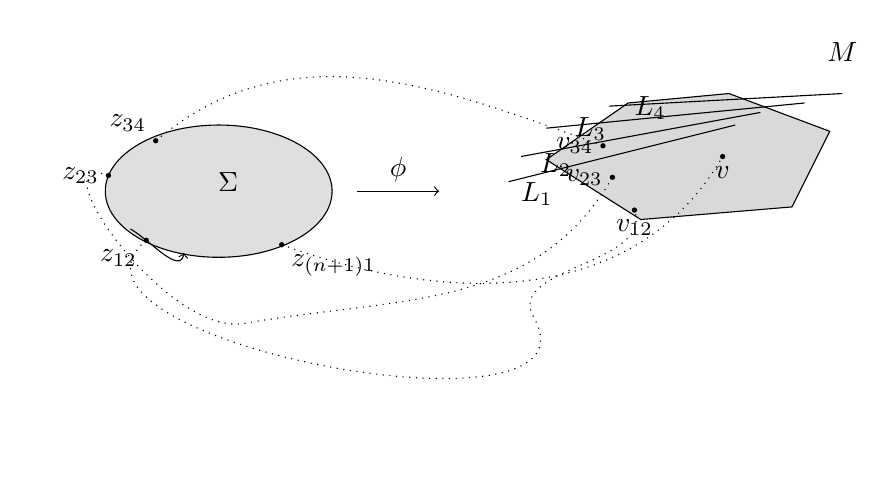
\begin{tikzpicture}[scale=0.8]
  % 左：圆盘 Sigma
  \fill[gray!25] (0,0) ellipse (1.8 and 1.05);
  \draw (0,0) ellipse (1.8 and 1.05);
  \fill (-1.0,0.8) circle (1.2pt) node[above left] {$z_{34}$};
  \fill (-1.75,0.25) circle (1.2pt) node[left] {$z_{23}$};
  \fill (-1.15,-0.78) circle (1.2pt) node[below left] {$z_{12}$};
  \fill (1.0,-0.85) circle (1.2pt) node[below right] {$z_{(n+1)1}$};
  \node at (0.15,0.15) {$\Sigma$};
  \draw[->] (-1.4,-0.6) to[out=-30,in=-100] (-0.55,-0.98);
  % 映射 phi
  \draw[->] (2.2,0)--(3.5,0) node[midway,above] {$\phi$};
  % 右：M 中的多边形
  \fill[gray!30] (5.2,0.5)--(6.5,1.4)--(8.1,1.55)--(9.7,0.95)--(9.1,-0.25)--(6.7,-0.45)--cycle;
  \draw (5.2,0.5)--(6.5,1.4)--(8.1,1.55)--(9.7,0.95)--(9.1,-0.25)--(6.7,-0.45)--cycle;
  \node[above] at (9.9,1.9) {$M$};
  \draw (4.6,0.15)--(8.2,1.05); \node at (5.05,-0.05) {$L_1$};
  \draw (4.8,0.55)--(8.6,1.25); \node at (5.35,0.42) {$L_2$};
  \draw (5.2,1.0)--(9.3,1.4); \node at (5.9,0.98) {$L_3$};
  \draw (6.2,1.35)--(9.9,1.55); \node at (6.85,1.32) {$L_4$};
  \fill (6.6,-0.3) circle (1.2pt) node[below] {$v_{12}$};
  \fill (6.25,0.22) circle (1.2pt) node[left] {$v_{23}$};
  \fill (6.1,0.72) circle (1.2pt) node[left] {$v_{34}$};
  \fill (8.0,0.55) circle (1.2pt) node[below] {$v$};
  % 虚线连接
  \draw[dotted] (-1.0,0.8) to[out=40,in=160] (6.1,0.72);
  \draw[dotted] (-1.75,0.25) to[out=160,in=190] (0.4,-2.1) to[out=10,in=-120] (6.25,0.22);
  \draw[dotted] (-1.15,-0.78) to[out=-140,in=-60] (5.0,-2.0) to[out=120,in=-70] (6.6,-0.3);
  \draw[dotted] (1.0,-0.85) to[out=-20,in=-120] (8.0,0.55);
\end{tikzpicture}
\end{center}

% [原文 p.11]
当 $(M,\omega)$ 是某个可微流形 $B$ 的余切丛时，Fukaya 范畴 $\mathit{Fuk}(M,\omega)$ 与 $B$ 上的 Morse 同伦论的 $A_\infty$ 范畴之间有密切关系，彼此给出同一理论的不同解释 [14]；这一点有可能成为关于同调镜像对称根本理解的解决之钥（cf.\ [1], [27] 及其参考文献）。另一方面，在物理上，Fukaya 范畴以某个拓扑弦论为背景（1.4.4 节）。

\subsection{范畴论的对偶性}

从空间之上所承载的代数结构来把握空间所具有的性质，这使几何学灿烂地发展起来。例如，在旨在构建新空间概念的非交换几何中，以拓扑空间与其上的连续函数环之间的等价性（Gelfand–Naimark 定理）为基础，把一般的非交换环看作确定了以之为函数环的「非交换空间」的东西，以此作为出发点。代数几何也是以同样的空间与环的对应为基本之一的学问。可微流形上的微分形式所附随的 $A_\infty$ 结构（cf.\ 1.3.2 节）也可看作同样的方向性。

范畴也是代数的扩张。范畴的对象上的态射的集合构成幺半群（定义了积结构的集合），而域 $K$ 上加法范畴中对象上的态射所构成的 $K$ 向量空间构成 $K$ 代数。因此，在辛流形上考虑 Fukaya 范畴（1.3.3 节），或在复流形上考虑相干层所构成的范畴（1.3.1 节），都可以说是在这一潮流之上的。最近在代数几何中，研究空间上的范畴的结构有时也被称为非交换代数几何。

这一潮流尤其因 Kontsevich 的同调镜像对称猜想 [37] 而被激活。一般地，镜像对称性主张某个辛流形 $(\hat{M},\omega)$ 上的某种结构与复流形 $(M,J)$ 上的某种结构之间的等价性；特别地，同调镜像对称猜想主张这些范畴论中同调代数结构的等价性

\[\Tr(\mathit{Fuk}(\hat{M},\omega))\simeq\Db(\mathit{coh}(M,J))\]

对这一等式的说明大概需要一些篇幅。Fukaya 范畴 $\mathit{Fuk}(\hat{M},\omega)$ 是应当作为 $A_\infty$ 范畴来形式化的东西，而导出范畴是三角范畴。要比较两者，必须把两者放在同一框架中处理。正因如此，Kontsevich 提出了一般地从 $A_\infty$ 范畴构造三角范畴的方法 [37]。这是作为 Bondal–Kapranov 由 DG 范畴构造三角范畴之方法的自然推广而得到的。如此从 Fukaya 范畴 $\mathit{Fuk}(\hat{M},\omega)$ 得到的三角范畴记作 $\Tr(\mathit{Fuk}(\hat{M},\omega))$。一般地，按 1.3.1 节所述构造从阿贝尔范畴得到的东西称为导出范畴，但按此方法从 $A_\infty$ 范畴 $\cC$ 得到的三角范畴 $\Tr(\cC)$，有时也称为导出 $A_\infty$ 范畴，或 $\cC$ 的导出范畴等。如此，主张 Fukaya 范畴与相干层的范畴作为三角范畴的等价，正是同调镜像对称的（原本的）一种形式化。

% [Tutor Note: 术语锚点：$\Tr(-)$ 是三角包络（triangulated envelope），见 5.5.2 节（Bondal–Kapranov 由 DG 范畴构造）与 7.3.1 节（由 $A_\infty$ 范畴构造）。此处 $\Tr$ 并非迹（trace），记号按原书排印，阅读时注意与「迹」区分。]

% [原文 p.12]
本书在 5.5.2 节说明 Bondal–Kapranov 由 DG 范畴构造三角范畴的方法，在 7.3.1 节说明由 $A_\infty$ 范畴构造三角范畴的方法。

在各种例子中，已讨论了在各种层面上同调镜像对称成立。（并非所有论文都以三角范畴的等价来讨论。）例如，椭圆曲线（带复结构的环面 $T^2$）的镜像对偶是某个辛环面（带辛结构的 $T^2$）。以这种情形为首的 Calabi–Yau 流形，以及 Fano 流形与其镜像对偶的辛流形等情形下的同调镜像对称，已有若干肯定性的讨论（[1], [20], [27] 的参考文献）。然而，不仅有许多尚未得到实证的例子，而且若把「这样的对偶性为何存在？」这一根本理解也包括进来，则这样的研究还只能说刚刚开始。

\section{与弦理论的关系}

\subsection{弦理论}

作为物理背景，同调镜像对称的设定对应于拓扑弦论中 tree 开弦的理论 [1], [20]。

一般地，弦理论是指好的对称性之 Riemann 面 $\Sigma$ 上的场论。Riemann 面是 1 维复流形，但作为实流形是 2 维曲面，它描述由 1 维弦的时间演化所作出的 2 维面。$\Sigma$ 上的场是 $\Sigma$ 上函数的推广，一般是指到某个适当的值域 $X$ 的映射 $\phi : \Sigma\to X$。（当 $X=\R$ 时，$\phi$ 是 $\Sigma$ 上的函数。）指定场的种类（粒子的种类），并指定这些场的泛函（称为作用泛函）之一，就指定了一个场论。

描述在某个流形 $M$ 中运动的弦的场论，作为场包含映射 $\phi : \Sigma\to M$。进一步，当 $M$ 具有附加结构、例如辛结构、复结构等时，可定义包含这些信息的作用泛函。如此，场论反映了 $M$ 的几何信息。

弦理论中最基本的量是弦的散射振幅（表示弦相互作用、即多条弦入射而不同的多条弦出射之概率的量）。散射振幅由决定 Riemann 面上的场论以及与之相适的带点 Riemann 面的模空间的紧化而得到，并作为该紧化模空间上的某个积分给出。应当考虑的最一般的 Riemann 面具有亏格、多条边界 $S^1$，并在 Riemann 面内部及其边界 $S^1$ 上带点；内部的点与边界上的点分别对应闭弦、开弦的状态之插入。

% [Tutor Note: 可验证锚点（作用泛函）：取 $X=\R$，则 $\phi:\Sigma\to\R$ 是 $\Sigma$ 上的函数，作用泛函是函数空间到数域的映射，例如 $S[\phi]=\int_\Sigma \dd^2 z\,\sqrt{g}\,g^{ab}\partial_a\phi\,\partial_b\phi$；本书不需要其具体形状，只需「场论 = 场 + 作用泛函」这一对应，见 p.12 同段。]

% [Tutor Note: 术语锚点：モジュライ空間 = 模空间 moduli space；コンパクト化 = 紧化 compactification；点付きリーマン面 = 带点 Riemann 面 pointed Riemann surface；散乱振幅 = 散射振幅 scattering amplitude。p.12 所说的「带点 Riemann 面的模空间」在 tree 开弦情形其紧化正是 Stasheff 多面体（p.13 明言），这是本书把弦论与 $A_\infty$ 结构联系起来的枢纽。]

% [原文 p.13]
由这些散射振幅确定的代数结构，由带点 Riemann 面的模空间之紧化的分层（stratification）所附随的特殊性质、一般地由拓扑 operad 等结构所支配。在这种意义上，弦理论就是带点 Riemann 面的模空间之紧化所构成 operad 的表示。

\subsection{弦理论与同伦代数}

由带点 Riemann 面的模空间之紧化所附随的 operad 上的表示而得到的东西，是称为同伦代数的一类代数。（不过，「同伦代数」一词的定义并未被精确确定。）

可以把带点 Riemann 面的种类限制为作为弦理论封闭的方式。例如，考虑仅开弦的理论（对应于只在边界上带点的 Riemann 面）时，对两个 Riemann 面，分别取其边界上的点并相互适当地接合而成的 Riemann 面仍然只在边界上带点。类似地，仅闭弦的理论（对应于不具边界的 Riemann 面）自身封闭。作为其他分类，可以考虑不含圈的 Riemann 面。Riemann 面的把手被视为闭弦的圈。类似地，具有两条以上边界的 Riemann 面被视为含有开弦的圈。这些圈被视为弦理论中的（在标的空间 $M$ 上的场论意义上的）量子效应。不含圈的理论称为 tree 理论，据认为它描述弦的（半）古典论。

tree 开弦的理论，即以带边界点的圆盘为 Riemann 面的理论，实际上确定 $A_\infty$ operad。事实上，作为带点圆盘的模空间之紧化，得到 Stasheff 多面体（cf.\ [32]）。因此，tree 开弦的理论构成 $A_\infty$ 代数。类似地，tree 闭弦的理论、即以带点球面为 Riemann 面的理论，附随有 $A_\infty$ 代数（＝同伦结合代数）的李代数版，即 $L_\infty$ 代数（＝同伦 Lie 代数）。不过，此时紧化的方式不止一种，需要考虑适合理论（Riemann 面上的场论）的紧化，有时也考虑称为 $\mathrm{Comm}_\infty$ 代数的结构。作为对应于 tree 开弦与 tree 闭弦混合系统的同伦代数，有 open-closed 同伦代数（OCHA）（cf.\ [32]）。这样的代数结构，例如在弦场论中已由 Zwiebach 讨论过。弦场论是指构造成使其作为场论的散射振幅再现弦理论的散射振幅的理论。用同伦代数的语言说，弦理论的散射振幅就是弦场论所定义的同伦代数的极小模型。如此，同伦代数是描述弦理论结构的自然框架。

对于含圈的弦理论，对应的代数结构框架之候补是存在的，但作为一般理论，目前还没有到能有效应用它们的阶段。

% [Tutor Note: 术语锚点：$L_\infty$ 代数 = 同伦 Lie 代数（homotopy Lie algebra），$\mathrm{Comm}_\infty$ 代数 = 同伦交换代数；与 $A_\infty$（同伦结合）的差别在于把结合律换成 Jacobi 恒等式（或交换律）。OCHA = open-closed homotopy algebra，见 [32]。这些词 glossary 未收，已列入回执。]

% [原文 p.14]
\subsection{D-膜范畴}

关于含开弦的理论，作为开弦的边界条件要考虑称为 D-膜的东西。含开弦的弦理论应当由 D-膜所构成的范畴来描述，这一般称为 D-膜范畴 [41]。虽说是范畴，却未必是通常意义的范畴；它以 D-膜为对象，并在它们之上考虑作为弦理论适当的结构。特别是目前，作为对应于 tree 开弦理论的东西，关于 D-膜范畴的 DG 范畴、或作为 $A_\infty$ 范畴 $\cC$ 的结构，研究十分活跃。在这一形式化中，$\cC$ 的 Møller–Cartan 方程是确定 DG 或 $A_\infty$ 结构的弦场论中的运动方程，而 $\cC$ 的扭曲复形被解释为运动方程的解、即「理论的真空」。这给出了 5.5.2 节、7.3.1 节中三角范畴的 DG 增广、$A_\infty$ 增广理论的物理说明。

当然，从弦理论的立场来看，把 D-膜范畴作为 $A_\infty$ 范畴处理只是最初的一步。首先获得对该 $A_\infty$ 范畴的充分理解是先决问题；不过，通过引入闭弦的结构来考虑范畴的族，或通过考虑包含圈的（对应于所有 Riemann 面的）弦理论的结构，D-膜范畴应当会被进一步「量子化」，这是不言而喻的。

% [Tutor Note: 可验证锚点（Møller–Cartan 方程）：在 DG 代数情形，方程为 $\dd m+\frac12[m,m]=0$；在 $A_\infty$ 代数情形，$\cC$ 的扭曲复形对应于元素 $m$ 满足 $\sum_k m_k(m,\ldots,m)=0$（即 $A_\infty$ 关系式的「元素版」），故「真空 = 扭曲复形」的对应可逐项核对。术语：捻り複体 = 扭曲复形 twisted complex（glossary 未收，列入回执）。]

\subsection{镜像对称性}

镜像对称性是辛流形与复流形（或代数簇）之间的对偶性，被理解为辛流形上的拓扑弦论即 A 模型与复流形上的拓扑弦论即 B 模型之间的等价性。另一方面，在这些 A 模型、B 模型各自之中，也大致可分为两种拓扑弦论。一种是通常意义上的与流形对应的弦论；另一种是对流形 $X$（例如复超平面 $\C^n$ 等亦可）上的多项式 $f$，对应于由 $f=0$ 所确定的空间的弦论。后者是以 $X$ 为标的空间、具有称为 Landau–Ginzburg（LG）势的多项式 $f$ 的拓扑场论，称为 LG 模型。已知前一种与后一种所确定的拓扑弦论之间也存在某种对偶性，称为 CY-LG 对应。这里 CY 是 Calabi–Yau 的缩写；由于把前一种类型的理论在 Calabi–Yau 流形情形下考虑是典型例子，故如此称呼，但实际上这一对应是对更一般的 Kähler 流形讨论的。总结起来，在 A 模型侧、B 模型侧各自之中，把前一种理论称为 $\sigma$（sigma）模型，则存在或期待如下对偶性。

% [Tutor Note: 术语锚点：ランダウ・ギンツブルグ（LG）ポテンシャル = Landau–Ginzburg 势；CY-LG 対応 = CY-LG 对应；ケーラー多様体 = Kähler 流形；タキオン凝縮 = tachyon 凝聚（tachyon condensation，见 p.15）。LG 模型的锚点：取 $f:\C^n\to\C$ 的多项式，$f=0$ 定义超曲面，其上的拓扑弦论与 $\C^n$ 上的 LG 模型（势 $f$）对偶，这是 CY-LG 对应的基本情形。]

\begin{center}
\begin{tikzpicture}[scale=1.0]
  \node[draw, minimum width=2.7cm, minimum height=0.8cm] (sa) at (0,2) {$\sigma$-A 模型};
  \node[draw, minimum width=2.7cm, minimum height=0.8cm] (sb) at (5.2,2) {$\sigma$-B 模型};
  \node[draw, minimum width=2.7cm, minimum height=0.8cm] (la) at (0,0) {LG-A 模型};
  \node[draw, minimum width=2.7cm, minimum height=0.8cm] (lb) at (5.2,0) {LG-B 模型};
  \draw[<->] (sa)--(sb);
  \draw[<->] (la)--(lb);
  \draw[<->] (sa)--(la);
  \draw[<->] (sb)--(lb);
  \draw[<->] (sa)--(lb);
  \draw[<->] (sb)--(la);
\end{tikzpicture}
\end{center}

% [原文 p.15]
更准确地说，在 LG 模型侧所处理的是带有特定群作用的东西；这 4 个并非全都已被完全定义，在讨论对偶性之前，如何形式化它们也是今后应当研究的问题之一。话虽如此，可以预期这些对偶性会在各种层面上、即从限制到 tree 闭弦、tree 开弦等的情形，到含圈的开弦与闭弦混合的弦理论中，被形式化并成立。特别地，与同调镜像对称相关的、（D-膜范畴中）tree 开弦结构的数学形式化如下。首先 A 模型侧无论哪种都要考虑 Fukaya 范畴，其中 LG-A 模型特别地由 Seidel 研究过 [49]，故有时也称为 Fukaya–Seidel 范畴。在 $\sigma$ B 模型中，考虑相干层的导出范畴，其背后有三角 DG 范畴的结构。关于 LG-B 模型，有矩阵因子化所构成的 DG 范畴，以及作为其同伦范畴得到的三角范畴 [1], [30], [52]。如此，直接地说，三角范畴的结构是在 B 模型侧讨论的。三角范畴中同调代数的、在拓扑弦论中由 tachyon 凝聚给出的物理解释也存在；受这些讨论启发，三角范畴中稳定性的概念也被形式化并正在推进研究 [1]，但在本书中未能涉及这一点。

% [Tutor Note: 术语锚点（p.15）：行列因子化 = 矩阵因子化 matrix factorization；tachyon 凝聚 = tachyon 凝聚 tachyon condensation；三角 DG 圏 = 三角 DG 范畴（glossary 已有）。注意原书 p.15「$\sigma$ B 模型」处 L 与 G 之间无连字符，与图及 p.14 的「B 模型」写法略异，本译本统一作「$\sigma$ B 模型」。]

\section{范畴论中的技术侧面}

\subsection{「同构」这一概念}

一般地，比较两个集合时要考虑它们之间的映射；同样地，在范畴中比较两个对象时，要考虑它们之间的态射。特别地，当对象 $X,Y$ 之间存在满足

\begin{equation}
g\circ f=\id_X,\qquad f\circ g=\id_Y \tag{1.3}
\end{equation}

的态射 $f : X\to Y$, $g : Y\to X$ 时，称 $X,Y$ 同构（isomorphic）（定义 4.7）。在几乎所有的数学中，同构的对象都被视为同一。对于本书所处理的概念，也要注意有几个是在模去同构（及其任意性）之下定义的。例如用泛性质定义的东西（cf.\ 1.5.4 节）、三角范畴中例外对象系的变异（定义 5.64）等即属此类。

% [Tutor Note: 锚点：式 (1.3) 就是范畴中同构态射的定义。可验证例：$\Set$ 中同构即双射；$\Ab$ 中同构即群同构；而在一般范畴中，$f$ 有双侧逆这一条件严格强于「$f$ 单且满」，例如在环范畴中单态射不必是同构。另「例外的対象系の変異」= 例外对象系的变异（mutation of an exceptional collection），其定义依赖同构意义下的选取，故 p.15 把它列为「模同构定义」的例子。]

\subsection{同伦等价与局部化}

对于拓扑空间，我们考虑其同调；同样地，对于范畴 $\cC$，也希望从中抽出适当的信息。正因如此，本书考虑范畴论中的同调代数。因此，作为范畴 $\cC$，主要考虑同调代数操作能良好定义的加法范畴、阿贝尔范畴。

% [原文 p.16]
对范畴 $\cC$，$\cC$ 的复形所构成的范畴 $\Comp(\cC)$ 虽然由莫大数量的对象构成，但它是由 $\cC$ 唯一确定的，所以作为信息并未增加。然而，用同构类对全部复形进行分类一般信息量过大。反之，若用复形的上同调的同构类分类，则舍弃的信息又过多。

作为从复形提取基本信息的手段，一般能想到两个处于这两者之间的重要方法。其一是用某个等价关系去除态射空间。由此，在取商之前阶段并非恒等态射 $1_X$ 的东西，在取商之后可能与 $1_X$ 等价，原本不同构的东西可能变得同构。作为这样的等价关系，有同伦等价关系。

要在对象之间定义称为同伦等价的等价关系，通常首先定义对象之间的映射之间的同伦。也就是说，当对象 $X,Y$ 之间的两个映射 $f,g : X\to Y$ 满足某个条件时，称 $f$ 与 $g$ 同伦，记作 $f\overset{\mathrm{h.e.}}{\sim}g$。作为该条件，考虑关于映射的合成表现良好的条件。此时，称对象 $X,Y$ 同伦等价，是指存在

\[[f]\in\{X\to Y\}\big/\overset{\mathrm{h.e.}}{\sim},\qquad [g]\in\{Y\to X\}\big/\overset{\mathrm{h.e.}}{\sim}\]

且满足

\[[g]\circ[f]=[\id_X]\in\{X\to X\}\big/\overset{\mathrm{h.e.}}{\sim},\qquad [f]\circ[g]=[\id_Y]\in\{Y\to Y\}\big/\overset{\mathrm{h.e.}}{\sim}\]

时。换言之，即存在 $f : X\to Y$, $g : Y\to X$ 使 $g\circ f\overset{\mathrm{h.e.}}{\sim}\id_X$, $f\circ g\overset{\mathrm{h.e.}}{\sim}\id_Y$。

% [Tutor Note: 原文 p.16「写像の合成に関してうまくふるまうものもを考える」中「ものもを」疑衍一「も」（正誤表未收，疑为排印重复），本译本按语义译出。术语：h.e. = homotopy equivalent（同伦等价），记号 $\overset{\mathrm{h.e.}}{\sim}$ 表示同伦关系；注意 $[f]$ 表示同伦类，故取商后才有 $[g]\circ[f]=[\id_X]$ 的陈述。]

另一方面，如果有扩大态射空间的方法，那么由此也可能增加互相等价的东西。事实上，态射增多，使合成 $g\circ f$ 成为恒等态射的 $f,g$ 存在的可能性也就增大。作为扩大态射空间的基本操作，有局部化（4.7 节）。这是环的局部化（2.2.6 节）向范畴论的扩张。

\subsection{态射的提升}

在范畴论中，对象不过是单纯的标号；对象 $X$ 的性质，采取通过观察它与其他对象之间的态射的性质来看的立场。特别是在本书也要展开的范畴论同调代数中，讨论关于态射的各种性质。此时最频繁出现的问题如下。

给定态射 $f : X\to Y$, $g : Z\to Y$ 时，是否存在满足 $f=g\circ h$ 的态射 $h : X\to Z$？

% [原文 p.17]
\begin{center}
\[\begin{tikzcd}[row sep=2.4em, column sep=2.8em]
  & Z \arrow[d,"g"] & & & Z \arrow[d,"g"] \\
  X \arrow[r,"f"] & Y & \Longrightarrow & X \arrow[r,"f"'] \arrow[ur,dashed,"h"] & Y
\end{tikzcd}\]
\end{center}

当这样的态射 $h$ 存在时，说态射 $f : X\to Y$ 经过 $Z$，或经过 $g : Z\to Y$。

这个问题也是代数拓扑中的基本问题；当这样的 $h$ 得到时，也常说得到了态射 $f$ 的提升。在本书中，当用交换图表陈述从某个对象到另一个对象的态射之存在时，可以说绝大多数情形都是反复使用这种态射的提升、或把其方向全部反过来者来证明的。

% [Tutor Note: 术语锚点：リフト = 提升 lift。把 p.17 图中箭向全部反过来得到的是「扩张问题」（extension problem）：给定 $f:Y\to X$, $g:Y\to Z$，求 $h:Z\to X$ 使 $h\circ g=f$。本书第 5 章证明三角范畴公理 (Tr3)、(Tr4) 时反复使用的正是这两种形式；可验证锚点：定義 4.25（积与余积）的对偶论证即是「方向全部反过来」的最简例子。]

\subsection{泛性质}

本书中频繁出现「泛性质」一词。例如，集合的直和、直积（引理 2.3），加法群（或 $R$ 模）之间的直和、直积（引理 2.62），张量积（命题 2.64, 2.68, 2.70），环的局部化（定理 2.43），范畴的局部化（定理 4.58）等，都由某个泛性质所刻画。这种关于泛性质的讨论的共同点在于：具有某个泛性质的数学对象，只要存在，就在由这些数学对象所构成的范畴中、模去同构对象的意义下必定被唯一确定。也就是说，导出这种结果的性质被称为泛性质。关于集合的直和、直积，加法群或 $R$ 模之间的直和、直积，张量积，环或范畴的局部化等所具有的泛性质，具有该泛性质的数学对象的唯一性可用完全类似的论证证明。因此，证明虽有省略的部分，但例如看集合的直和、直积的情形（引理 2.3），其他情形也就能明白。

这样的泛性质在一般范畴中定义各种运算。例如，定义范畴 $\cC$ 中的直积、直和（定义 4.25）。在一般范畴中直积、直和未必存在，但存在时在模同构的意义下被唯一确定。当然，当 $\cC$ 是集合所构成的范畴 $\Set$、加法群所构成的范畴 $\Ab$ 等时，直积、直和存在，且与先前所讨论的一致。4.3 节用泛性质定义加法范畴 $\cC$ 中态射的像（image）、核（kernel）等。

对于某个对象，泛性质一般是关于与 $\cC$ 的所有对象之间的态射的性质。另一方面，范畴论是认为对象自身不过是单纯的标号、通过观察对象之间态射的性质来理解事物的学问。在这个意义上，可以说泛性质是恰好契合范畴论之概念的想法。

% [Tutor Note: 泛性质唯一性的论证模板（补出作者省略的细节）：若对象 $P$ 与 $P'$ 都满足同一泛性质，则由泛性质分别得到唯一的态射 $P\to P'$ 与 $P'\to P$；再对 $P$（或 $P'$）自身应用泛性质，知这两个态射的合成必为恒等态射，故 $P\cong P'$。可验证的最简例子：集合的直积 $A\times B$ 满足「对任意 $X$，$\Hom(X,A\times B)\cong\Hom(X,A)\times\Hom(X,B)$」，由这一条即可反推投影映射的唯一性。]
